\documentclass[a0,portrait]{a0poster}
\usepackage{multicol}
\usepackage{poster}
\usepackage{amsmath,amsthm,amssymb}
\usepackage{epstopdf}
\usepackage{xspace}
\usepackage{verbatim}
%\usepackage{sagetex}
\usepackage{circuitikz}

%\usepackage{pst-all}
%\usepackage{pst-circ}

\usepackage{titlesec}
\titlespacing*{\subsubsection}{0pt}{*2}{*0}
\titlespacing*{\subsection}{0pt}{0pt}{*0}

\newcommand{\Bold}{\mathbf}

\title{Homomorphic Cryptosystems}

\author{
Jeremy Caci, Ali Hajy, Jonah Jolley\\
Clark Rinker, Philip Robinson\\
Advisor : Dr. David Bover\\
Computer Science Department
}



\begin{document}
\maketitle

\def\fh{{\em Fully Homomorphic\xspace}}

\begin{multicols}{2}
\begin{slide}{Abstract}

We present a formal inquiry of the first fully homomorphic encryption scheme proposed by Craig Gentry in 2008. Moreover we introduce the first implementation of this cipher in the Python programming language. A fully homomorphic encryption scheme enables the execution of arbitrary operations on encrypted data without the decryption key which, put simply, allows for a third party to  store and manipulate sensitive information without the ability to interpret it. 
\parskip 1em

The applications of an efficient fully homomorphic encryption system are potentially limitless. A contemporary example is cloud based email, where a decentralized server stores and serves encrypted user email. Furthermore, such a system would allow for users to request the server to perform search queries on stored data without loss of privacy. This is a particularly enticing scenario given the recent boom in portable devices and multiparty computation, both of which currently have serious security concerns. 

Our investigation includes a high level synopsis of the mathematics involved in fully homomorphic encryption, a complete demonstration of our implementation in Python, and finally a overview of the space and asymptotic time complexities of the proposed system. 

\end{slide}

\begin{slide}{Definitions}
In order for a cryptographic system to be considered \fh we need to make some clear definitions availible. It also proves benificial to clearly express why these terms are significant and their relationships to eachother. 

\begin{itemize}
\item Circuit Operations
\begin{itemize}
\item Fundamental Gates

  The most basic logical operations; AND, OR, and NOT. 
%\item Polynomials
\end{itemize}
\item Bootstrapping

  Re-encrypting already encrypted data using elements from the original encryption circuit.
\begin{itemize}
\item Compact
%\item Circular Security
\end{itemize}
\item Secure Problems
\begin{itemize}
\item Approximate GCD
<<<<<<< HEAD
\item Subset Sum Problem 

  Given a set of rationals, is there a non-empty set whose sum is equal to $S$ where $S$ is a random integer. In this encryption scheme, $S$ is used as the secret key.
\item Computational Complexity
=======
\item Subset Sum Problem
  Given a set of integers, is there a non-empty set whose sum is $S$ where $S$ is a random integer that acts as the secret key.
%\item Computational Complexity
>>>>>>> 2b292a1455d7dbf8b87c23d0c705aa379e958d66
\end{itemize}

\end{itemize}


We may need to additionally add information about Rings, Prime Ideals, this can be added later. There are likely other definitions that are needed, and will likely be found as the ones above are addressed
\end{slide}


\begin{slide}{Circuit probably moved}

%\begin{comment}
\begin{multicols}{3}
\resizebox{\columnwidth}{!}{
\begin{circuitikz}\draw
(0,0) node[and port,scale=2.5] (myand) {}
(myand.in 1) node[anchor=east] {\({b_0}\)}
(myand.in 2) node[anchor=east] {\({b_1}\)}
(myand.out) node[anchor=west] {\({b_0 \cdot b_1}\;(\text{mod }2)\)}
;\end{circuitikz}
}

\resizebox{\columnwidth}{!}{
\begin{circuitikz}\draw
(0,0) node[xor port,scale=2.5] (myand) {}
(myand.in 1) node[anchor=east] {\({b_0}\)}
(myand.in 2) node[anchor=east] {\({b_1}\)}
(myand.out) node[anchor=west] {\({b_0 + b_1}\;(\text{mod } 2)\)}
;\end{circuitikz}
}

\resizebox{\columnwidth}{!}{
\begin{circuitikz}\draw
(0,0) node[not port,scale=2.5] (not) {}
(not.in) node[anchor=east] {\({b_0}\)}
(not.out) node[anchor=west] {\(1-{b_0}\;(\text{mod } 2)\)}
;\end{circuitikz}
}
\end{multicols}
%\end{comment}


\resizebox{\columnwidth}{!}{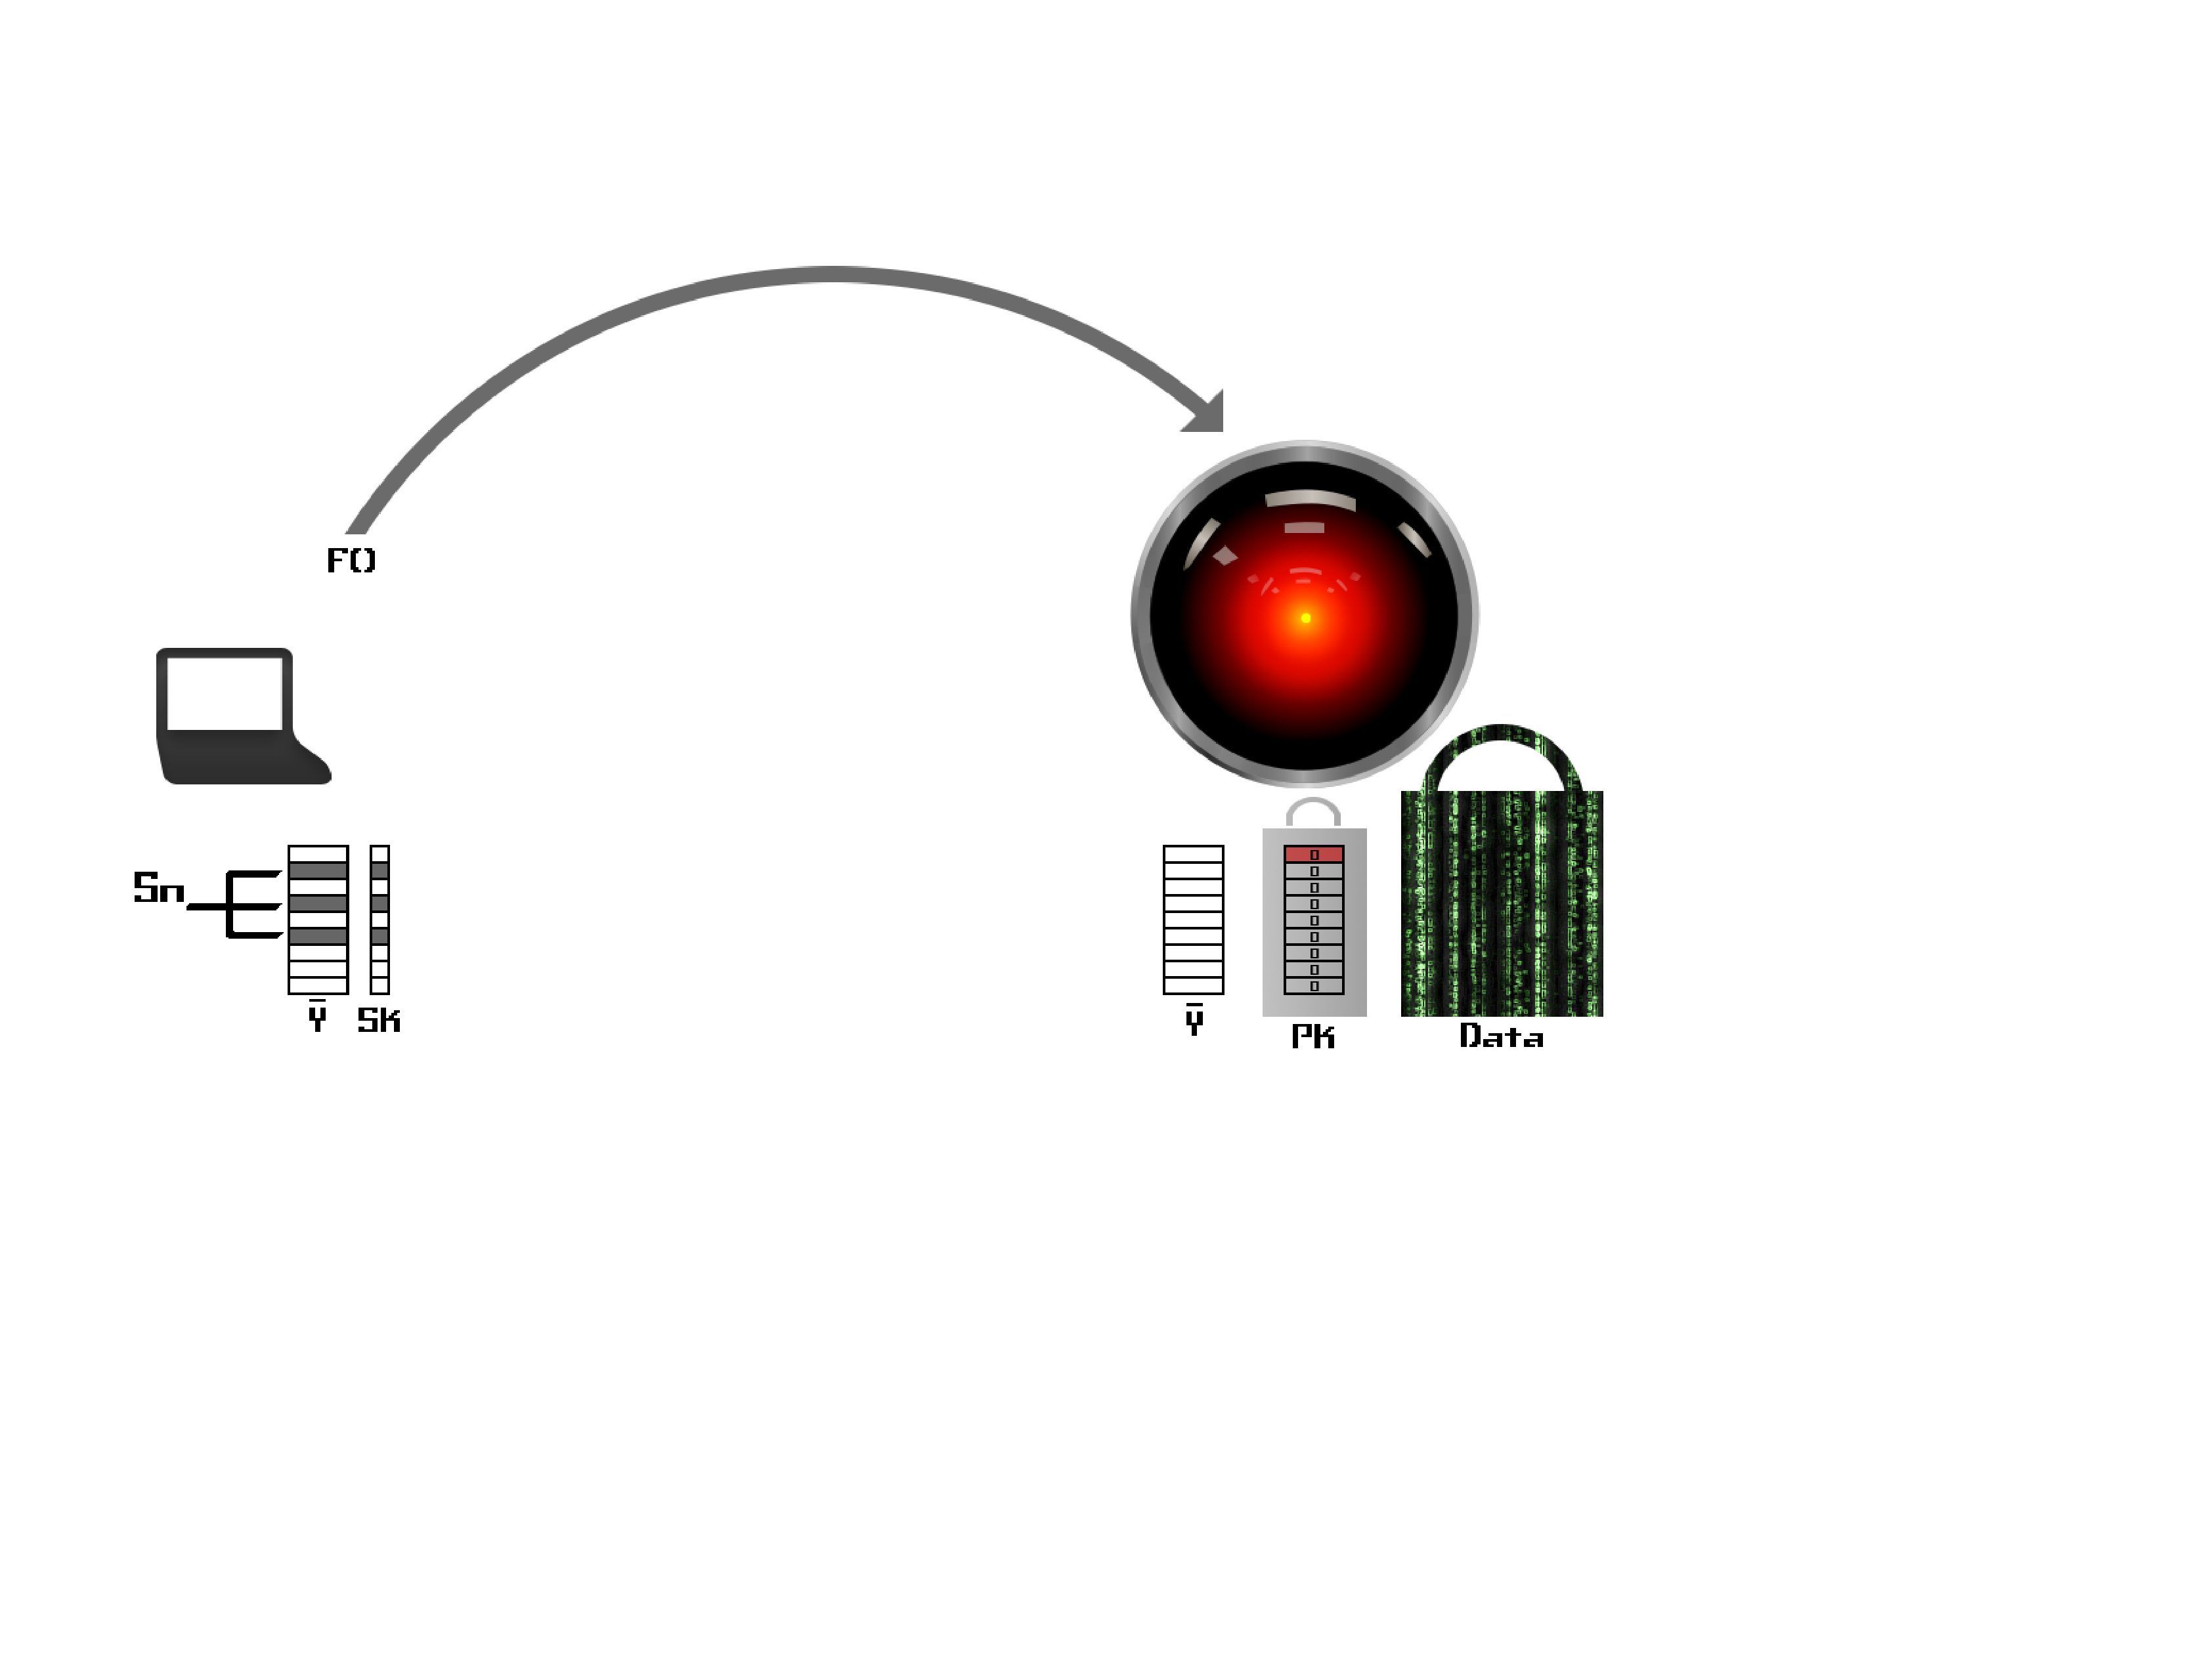
\includegraphics{infograph.eps}}
\end{slide}



\begin{slide}{Limitations}
\subsection*{Space Complexity}
  This cryptographic model has not yet been refined to a practical level. Encrypting data bitwise under these methods, such that the cipher text is cryptographically secure requires a great degree of noise/bloat to hide the pairity of our unencrypted message bidgit. 
\parskip 1em


 % \vspace{1em}
\resizebox{\columnwidth}{!}{
  \begin{tabular}{c|c|c|c|c|c}
     & {\small bit-size} &  {\small encrypted volume}  & \(\lambda = 8\) & \(\lambda = 16\) & \(\lambda = 64\) \\\hline 
    {\small bidgit} & 1 & \(\approx \lambda^7 \) & \(\approx\) 256 KB & 32 MB & 512 GB \\\hline
    {\small ``cadadr''} & 6 Bytes & & \(\approx\) 12 MB & 1.5 GB & 24 TB \\\hline
    {\small Declaration of Independence} & 8.5 KB & & \(\approx\) 17 GB & 2.1 TB & 34 PB\\
  \end{tabular}
  }%\end{center}
 % \vspace{1em}

  What we also notice is that the storage space of encrypted data is linear \(\;\in\Theta(1)\) with respect to information size.  It is also important to note that operations can as much as double the space complexity over the addressed space, but this is often not over a large block of space.

\begin{comment}
\begin{align*}
f_{(1\text{ bit},64)}&=512\; GB\\
f_{(6\text{ Bytes},64)}&=(512\; GB)\cdot6\cdot 8\\&=24\; TB
\end{align*}
\end{comment}

\subsection*{Cannot Evaluate Conditional Branching}
For any operation, if we are unable to 

\end{slide}

\begin{slide}{Security}

Given \(\lambda\) as a security Parameter 

we have a private key space of \(2^{(\lambda^2-2)} - (2^{\lambda^{2-1}})-1\)

The cryptographic hint uses the subset sum problem over a sparse subset. cracking the hint takes up space 

\[\left(\begin{matrix}\beta = \lambda^5\\\alpha \end{matrix}\right)\approx \beta^\alpha\] produces


The problem of cracking is {\em Soft NP-Complete}

%This is because as the security parameters grows, the searchspace and the cost of the operations grow. 
\end{slide}



%\end{multicols}
%\begin{multicols}{3}
\begin{slide}{Next Steps}
  What we have accomplished is effective but not efficient. Although we recognize that this cryptographic system is not a practical one, we would like to make it as realistic as possible. Because we are dealing with voluminous data, we are planning to distribute the storage and operations load accross an entire lab using {\em Hadoop} distributed systems. 
\parskip 1em 

  Because we are working with such large numbers, it is additionally very time-expensive to perform multiplication. The kids multiplication algorithm is \(\in\Theta(n^2)\), but even with Karatsuba's algorithm \(\approx\Theta(n\cdot\lg n)\) implemented in python we do not recieve sufficient speed up. We are planning to shuffle this task onto the video card of each machine using {\em PyCuda}, so that we can perform faster DFTs. By doing this we can gain speed in parallelization that we are normally unable to recieve with python derivatives.

  Finally, we are looking at shrinking our space complexity by migrating to supporting an n-ary system rather than a binary system. This means we'll need to more formally address definitions for our co-sets and ideals.% under \(\mathbb{Z}_{<+,\cdot>}\)
\end{slide}

\begin{slide}{Mathematical Background}
Describing the abstract Ideals relations
\end{slide}

\begin{slide}{Bootstrapping}
The Power of Bootstraping
\end{slide}

\begin{slide}{System Resources}
Memory Used for Project \\ Time to complete \(O(n)\) equivelent operation \\ Projected Space \\ Keysize 
\end{slide}

\begin{slide}{Significant Difficulties}

\end{slide}

\begin{slide}{Conclusion}
Our Findings \\ Further Implementations \\ Python as a Vehicle
\end{slide}
\begin{slide}{Circuit Diagram To Be Moved}

%\begin{comment}
\begin{circuitikz}[scale=2.5]\draw
% begin string compare
(0,6) node[xor port,scale=2.5] (myxor0){}
(myxor0.in 1) node[anchor=east] {\(s_0\)}
(myxor0.in 2) node[anchor=east] {\(c_{8\cdot i}\)}

(0,4) node[xor port,scale=2.5] (myxor1){}
(myxor1.in 1) node[anchor=east] {\(s_1\)}
(myxor1.in 2) node[anchor=east] {\(c_{8\cdot i + 1}\)}


{ [dotted, ultra thick] (-1,3) -- (-1,1) }

(0,0) node[xor port,scale=2.5] (myxorn){}
(myxorn.in 1) node[anchor=east] {\(s_{8\cdot n}\)}
(myxorn.in 2) node[anchor=east] {\(c_{8\cdot i + 8\cdot n}\)}

(2,3) node[nor port,scale=2.5] (myor) {}
(myxor0.out) -| (myor.in 1) {}
(myxorn.out) -| (myor.in 2) {}
(myxor1.out) -| (myor.in 1) {}
% begin carry adder
;\end{circuitikz}
%\end{comment}

\end{slide}


\begin{slide}{Bibliography}
Thats where the bibliography goes
\end{slide}
\end{multicols}
\end{document}
